\documentclass{article}

\usepackage{tikz}

\usetikzlibrary{automata,
    positioning,
    arrows,
    calc}

\begin{document}
\begin{center}
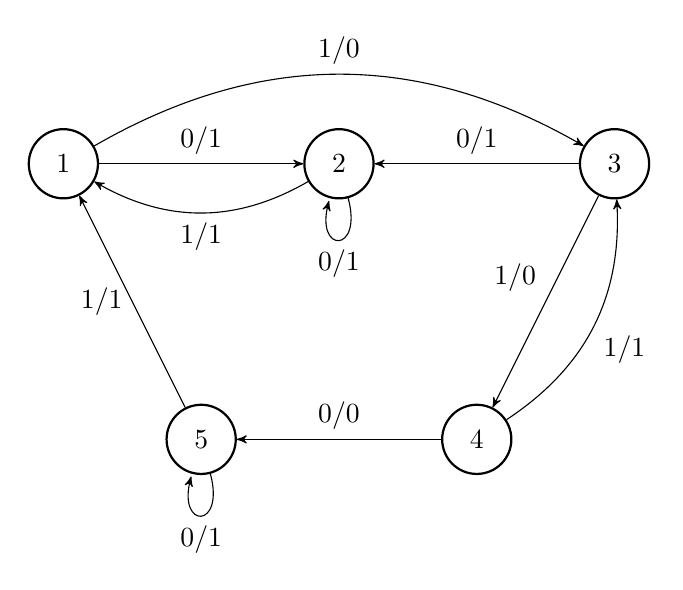
\begin{tikzpicture} [->,
    > = stealth',
    node distance = 3.5cm,
    every state/.style = {thick, fill = gray!0}]
\node[state] (q1) {$1$};  
\node[state, right of=q1] (q2) {$2$};  
\node[state, right of=q2] (q3) {$3$};  
\coordinate (midq2q3) at ($(q2)!0.5!(q3)$);
\node[state, below of=midq2q3] (q4) {$4$};  
\node[state, left of=q4] (q5) {$5$};

\draw (q1) edge[bend left, above] node{1/0} (q3);
\draw (q1) edge[above] node{0/1} (q2);

\draw (q2) edge[bend left, below] node{1/1} (q1);
\draw (q2) edge[loop below] node{0/1} (q2);

\draw (q3) edge[above] node{0/1} (q2);
\draw (q3) edge[above left] node{1/0} (q4);
    
\draw (q4) edge[above] node{0/0} (q5);
\draw (q4) edge[bend right, below right] node{1/1} (q3);

\draw (q5) edge[loop below] node{0/1} (q5);
\draw (q5) edge[left] node{1/1} (q1);
\end{tikzpicture}
\end{center}
\end{document}